\section{Grundlegende Verfahren}
Gesichtserkennung ist eine der fortschrittlichen Verfahren in der maschinellen Bildverarbeitung und wird ständig weiterentwickelt. Darunter fallen neben der Detektion des Gesichtes auch deren Analyse wie Orientierung, Übereinstimmungen oder das Erkennen von Mimik wie beispielsweise das Lächeln von Personen zum auslösen einer Kameras.\\
Bei vielen Anwendungen ist der Stand der Technik ein Neuronales Netz beteiligt.
\subsection{Künstliches neuronales Netz}
Ein künstliches neuronales Netz besteht aus miteinander verknüpften künstlichen Neuronen. Jedes Neuron besitzt Eingangswerte und einen Ausgabewert.\\
Um die Ausgabe zu bestimmen, werden die einzelne Eingangswerte des Neurons individuell Gewichtet, mit einer Übertragungsfunktion zusammengefasst und mittels eine Schwellenwertfunktion das Ergebnis bestimmt.\\
Um die Parameter (Gewichtung und Funktionen) des Neurons zu bestimmen, werden diese zufällig initialisiert und anschließend so angepasst, dass es zu einer gegebenen Eingabe das gewünschte Ergebnis liefert und der Fehler über dem gesamten Trainingsdatensatzes minimal wird.\\
Soll ein gesamtes Netz trainiert werden, so wird jedes einzelne Neuron zufällig Initialisiert und anschließend so angepasst das der Fehler des Netzes auf dem Trainingsdatensatzes minimal wird.\\
\cite{Maschin_Neuron}
\subsection{Convolutional Neural Network (CNN)}
Die CNN definieren in vielen Anwendungsbereichen momentan der Stand der Technik. Sie sind eine Weiterentwicklung der neuronalen Netze die vor allem im Bereich Klassifizierung eingesetzt werden, unter anderem bei der Bild- und Spracherkennung. Der unterschied liegt bei der Verwendung von gewichteten Faltungen der Eingabe.\\
Durch die Faltung werden die Information aus den umliegenden Punkten eines Bereiches zusammengefasst und komprimiert an die nächste Schicht weitergegeben, um in der untersten Schicht alle vorhanden Informationen zusammenzuführen. 
Der Faltungskern kann je nach Anwendung beliebig gestaltet sein, so ist eine Glättung durch einen Gauß-Kernel oder Kantendetektion durch einen Kirsch-Operator möglich.\\
Ein CNN kann in zwei Bereiche aufgeteilt werden, Feature Extraktion und Klassifizierung. Bei der Feature Extraktion werden verschiedene Kernel und Komprimierung auf den Eingabeinformationen angewendet um sie für den zweiten Teil aufzubereiten.
Gelernt werden kann jeder einzelne Kernel für sich und die jeweiligen Bewertungen der Kernel und Neuronen.\\
\cite{pdf_CNN}\cite{wiki_CNN}
\begin{figure}
	\centering
	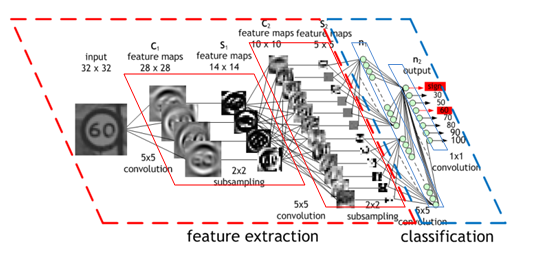
\includegraphics[width=0.7\linewidth]{img/cnn}
	\caption{Beispiel für den Aufbau eines CNN zur Klassifizierung von Zahlen \cite{bild_CNN}}
	\label{img_cnn}
\end{figure}
\subsection{Active Appearance Model (AAM)}
Dies ist ein Verfahren der Bildverarbeitung um Übereinstimmungen zu einem Modell zu finden. Dazu wird aus dem Trainingsdatensatz eine typische einheitliche Form des Objektes generiert mit seinen signifikanten Landmarks.\\
Soll nun zu einem Eingabebild die Übereinstimmung ermittelt werden, wird zuerst versucht es bestmöglich mittels Transformation in die typische einheitliche Form zu überführen. Sind dennoch Unterschiede vorhanden, liegt diese an der Erscheinung des Objektes.\\
\cite{wiki_AAM}
\subsection{Constrained Local Model (CLM)}
Dies ist ein Verfahren um mehrere Punkte eines Objektes zu lokalisieren. Dabei wird eine Wahrscheinlichkeitskarte für jeden einzelnen Punkt erstellt, wo dieser sich aufhalten kann, basierend auf der Ähnlichkeit des Punktes zur Darstellung im Bild. Nun wird versucht für das Bild, auf welchem gerechnet werden soll, für jeden Punkt den maximalen Wert zu erreichen zwischen passendem Farbverlauf und Wahrscheinlichkeit basierend auf der Position alle Punkte.\\
Dieser Art der Bestimmung von positionsabhängigen Punkten ist ziemlich zuverlässig und dennoch dynamisch genug um auch mit kleinen Veränderungen klar zu kommen.\\
Dies ist Wichtig, bei der Detektion von leicht verformbaren Objekten wie Gesichter und ist zuverlässiger als das Active Appearance Model (AAM).\\
\cite{pdf_CLM}
\subsection{Constrained Local Neural Fields (CLNF)}
Dabei handelt es sich um einen Gesichtsdetektor. Für die Detektion wird für jedes Merkmal ein eigener Detektor eingesetzt der auf einem Bildbereich arbeitet und eine Wahrscheinlichkeitskarte für dieses Merkmal erstellt.\\
Als nächster Schritt wird das Ergebnissen der Detektoren mit einer Karte der Position aller Landmarks mit ihren jeweiligen Abweichungen, kombiniert um somit die beste Position der Landmarks zu erhalten im Bezug auf den Farbverlauf und dem Verhältnis zu den anderen Landmarks.\\
\cite{CLNF}
\subsection{Non-maximum suppression  (NMS)}
Ein Verfahren um ein lokales Maximum zu bestimmen und kann z.B. in einem Bild eingesetzt werden um Kanten exakter zu bestimmen. Als Eingabe für das Verfahren im Beispiel, wird das Ergebnis eines Kantendetektor z.B. Kirsch-Operator verwendet. Dabei gibt die Höhe des Farbwertes eines Pixels an, wie nahe es an einer Kante im Originalbild liegen. Bei der Verarbeitung wird nun der Farbwert jedes einzelnen Pixels des Eingabebildes mit seinen umliegenden verglichen und sollte es nicht maximal sein auf Null gesetzt.\\
Auf diese Weise bleibt nur noch ein Kantenpixel übrig. Wird das Verfahren auf die Bestimmung von Boxen eingesetzt, so wird jene Fläche bestimmt die von allen am ehesten beschreiben wird.\\
\cite{NMS}\cite{wiki_Canny}
\subsection{Patch Experts}
Eine Bewertung, wie wahrscheinlich ein Landmark an einer bestimmten Position im Bild dargestellt ist. Dazu wird ein Bereich um die Position ausgewertet.\\
\cite{CLNF}
\subsection{Point Distribution Model (PDM) \& Generalized Adaptive View-based Appearance Model (GAVAM)}
Mit Point Distribution Model (PDM) können verformbare Objekte recht gut modelliert werden. Dabei wird die durchschnittliche Form $\overline{X}$ des Objekts anhand der Eingabe bestimmt und eine Matrix $P$ von Eigenvektoren ermittelt, um die möglichen Deformierungen darzustellen.
\begin{align*}
X &= \overline{X}+P\cdot b
\end{align*}
Somit kann durch einen Skalierungsvektor $b$ alle möglichen Eingabeformen $X$ des Objektes aus dem Durchschnittsmodell wiederhergestellt werden. Zur Vereinfachung reicht es, die signifikantesten Eigenvektoren in $P$ aufzunehmen und dennoch $X$ ausreichend genau beschreiben zu können.\\
Ist bekannt welche Art der Verformung durch den Eingenvektor dargestellt wird, z.B. eine bestimmte Orientierung, so kann anhand des Skalierungsvektors die Rotation der Eingabe bestimmt werden, siehe Generalized Adaptive View-based Appearance Model (GAVAM).\\
Eine Problematik bei dieser Art der Bestimmung der Rotation entsteht, wenn neben der Verschiebung der Landmarks durch die Rotation, auch eine Deformierung des Objektes stattgefunden hat und somit keine eindeutige Lösung gefunden werden kann. Dies ist eine Problem wenn auf Gesichtern gerechnet wird, da immer eine Veränderung der Mundwinkel oder Augenlider vorhanden ist.\\
\cite{pdf_PDM}\cite{pdf_GAVAM}\cite{wiki_PDM}